\documentclass[12pt]{article}
\usepackage[slovene]{babel}
\usepackage[utf8]{inputenc}
\usepackage[T2A]{fontenc}
\usepackage{amsmath}
\usepackage{amsfonts}
\usepackage{amssymb}
\usepackage[version=4]{mhchem}
\usepackage{stmaryrd}
\usepackage{graphicx}
\usepackage[export]{adjustbox}
\graphicspath{ {./images/} }
\usepackage{physics}
\usepackage{geometry}
\geometry{left=2cm,right=2cm,top=2cm,bottom=2cm}

\title{\textbf{Določanje Boltzmannove konstante}}
\author{Samo Krejan}
\date{maj 2025}

\begin{document}
\maketitle

\section{Uvod}

Boltzmanova konstanta $k_b$ je ena izmed najpomembnejših konstant v fiziki. Mi smo jo določali na podlagi diskusije o tokovih znotraj bipolarnega tranzistorja $(n-p-n)$. To so najbolj osnovni tranzistorji sestavljeni iz dveh $p-n$ stikov.

Naš bipolarni tranzistor ima tri kontakte imenovane kolektor, emitor in baza. V vaji kolektor in bazo kratko sklenemo in merimo kolektorski tok $I_c$ v odvisnosti od napetosti med bazo in emitorjem $U_{BE}$. Tevretična napoved te odvisnosti je podana z Ebbers-Mollovo enačbo:

\begin{equation*}
    I_c(T) = I_s(T)\left[\exp(\frac{e_0U_{BE}}{k_bT}) - 1\right],
\end{equation*}
kjer je $e_0$ osnovni naboj, $T$ temperatura in $I_s(T)$ velikost nasičenega toka v zaporni smeri.

Ker že v naprej vemo, da je Boltzmannova konstanta izredno majhna, vemo, da bo eksponent izredno velik in lahko \textit{pozabimo} na $-1$ saj je efektivna napaka zaradi tega manjša od procenta. Tako dobimo poenostavljeno enačbo \ref{ebermol}:

\begin{equation}
    I_c(T) = I_s(T)\exp(\frac{e_0U_{BE}}{k_bT}),
    \label{ebermol}
\end{equation}

Pri eksperimentu smo nadzorovali napetost med bazo in emitorjem s pomočjo baterije in variabilnega upora glej vezje \ref{vezje}, temperaturo pa smo nadzorovali s pomočjo Dewarjeve posode z vodo.

\begin{figure}[ht]
\begin{center}
    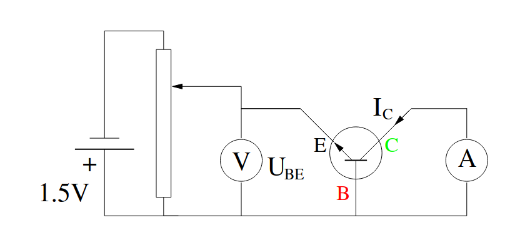
\includegraphics[width=10cm]{vezje.png}
    \caption{Skica vezja, uporabljenega skozi celotno vajo (vir: navodila)}
    \label{vezje}
\end{center}
\end{figure}


\section{Potrebščine}

\begin{itemize}
    \item bipolarni n-p-n tranzistor tipa BC182B,
    \item potenciometer in baterija (1,5 V),
    \item multimeter (Voltcraft 870) in namizni multimeter (SigLent SDM 3065X), žice,
    \item termometer, Dewarjeva posoda, grelec vode in izdelovalec ledu,
    \item prenosnik z ustrezno programsko opremo.
\end{itemize}

\section{Naloga}

\begin{enumerate}
    \item Izmerite odvisnost kolektorskega toka $I_c$ v odvisnosti od napetosti $U_{BE}$ pri temperaturah: 15, 35 in 55 stopinj,
    \item določite razmerje $e_0/k_b$,
    \item izmerite temperaturno odvisnost kolektorskega toka tranzistorja od temperature pri napetostih $U_{BE}$: 0,5 in 0,58 volta.
\end{enumerate}


\section{Rezultati in analiza}


\end{document}